\chapter{Preliminary Experimentation and results}

In order to evaluate the performance of the architecture, this system
is designed in two different modes, which is depicted in Fig
\ref{layout}.

% \begin{figure}[h]
%   \centering
%   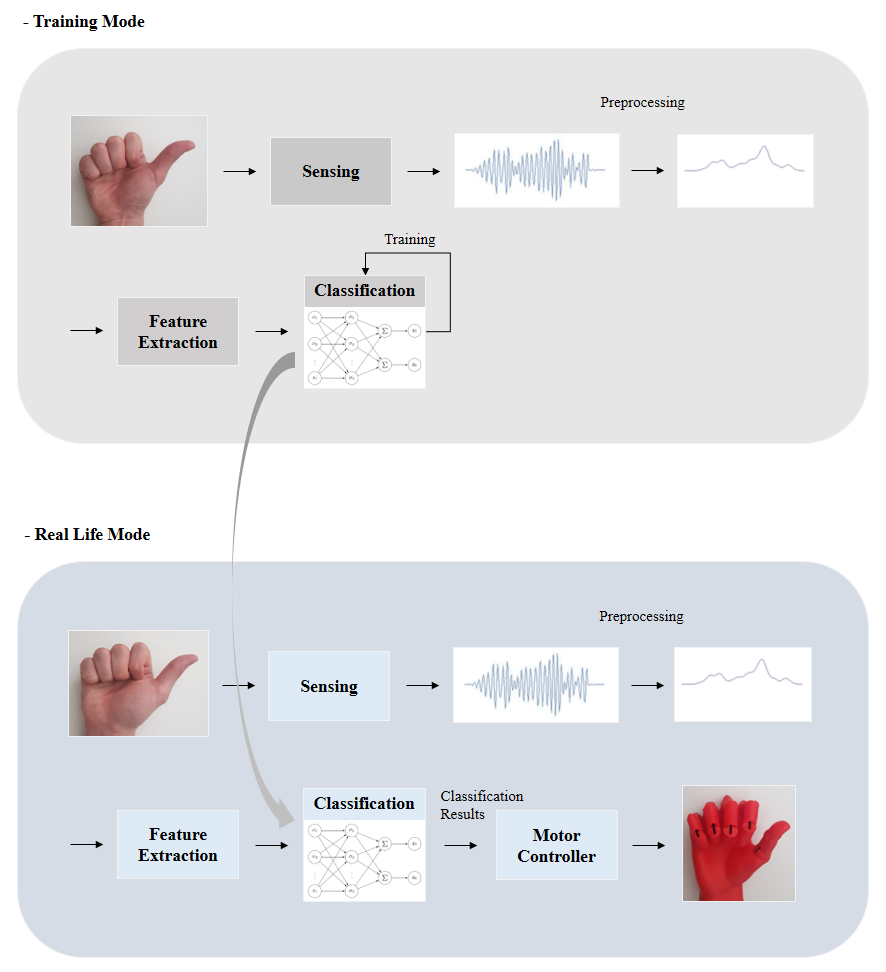
\includegraphics[width=3.5in]{Figures/layout_times.PNG}
%   \caption{Procedures of the system architecture.}
%   \label{layout}
% \end{figure}

\singlefigure[\textwidth]{layout}{layout_times.PNG}{Procedures of the system architecture}{Procedures of the system architecture}

In training mode, when the test subject group performs each different
action, 3 different EMG sensors read the subjects' muscle
contraction. The raw EMG sensor signals are rectified in real-time as
feature values for classification.  In real-life mode, the test
subjects perform the same actions to practically actuate the 3D
printed prosthetic hand. In this mode, sensing, preprocessing, and
feature extraction are processed, the same as in training
mode. However, this real-life mode predicts the subjects' actions
using a trained classification model to generate classification
results. This classification result is transferred to the motor
controller to control each motor assigned with each finger.

The experiments were conducted with $n=7$ test subjects containing 5
males and 2 females in their 20s and 30s. Each subject in the
experiment was instructed to attach three EMG muscle sensors to their
muscles, shown in Fig \ref{pic}.  The group was not composed of
amputees, though such individuals will be recruited for subsequent
experiments.  The placement of the three EMG sensor devices on the
forearm was chosen to accommodate amputees.

% \begin{figure}[h]
%   \centering
%   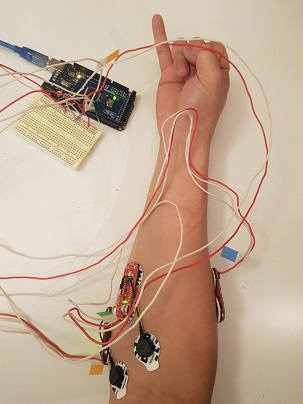
\includegraphics[width=2.5in]{Figures/am.jpg}
%   \caption{User's unique gesture (Pinky Swear) training with 3 EMG sensors}
%   \label{pic}
% \end{figure}

\singlefigure[.8\textwidth]{pic}{am.jpg}{User's unique gesture (Pinky Swear) training with 3 EMG sensors}{User's unique gesture (Pinky Swear) training with 3 EMG sensors}

The EMG muscle sensors are attached to the area of the flexor
digitorum superficialis, which is an extrinsic flexor muscle that
actuates four fingers with the interphalangeal joints, the flexor
digitorum profundus, which is the muscle that can bend the fingers to
grip, and the flexor pollicis longus, which actuates thumbs,
particularly for writing and painting.

To train various gestures into the prosthetic hand, a trial of using
the prosthetic hand with 3 EMG MyoWare Muscle Sensors was
performed. The subject tried to contract his muscles to perform his
intended hand behavior.  200 samples of EMG sensor data were recorded
during each action.

To testify to the decision-making algorithm's practicality, the
experiment routine is conducted for numerous behaviors, with the EMG
signals used to classify each different hand movement.

Each gesture is repeated, and simultaneously the 200 EMG muscle sensor
values are recorded when the user performs the motion as shown in
Table 1.

\begin{table}[ht]
\caption{Experiments with different actions} % title of Table
\centering % used for centering table
\begin{tabular}{c c} % centered columns (3 columns)
\hline\hline %inserts double horizontal lines
User behavior & Each iteration \\ [0.5ex] % inserts table
%heading
\hline % inserts single horizontal line
Hand Relax & 200 \\ % inserting body of the table
Clenching fist & 200 \\
Open hand & 200 \\
Thumbs up & 200 \\
Pointing somewhere & 200 \\
OK sign & 200 \\
Ball grip & 200 \\
Pencil grip & 200 \\
Smartphone grip & 200 \\
User's unique gesture (whatever the subject wants) & 200 \\ [1ex] % [1ex] adds vertical space
\hline %inserts single line
\end{tabular}
\label{table:nonlin} % is used to refer this table in the text
\end{table}


% \begin{singletable}{table:nonlin}{Experiments with different actions}{Experiments with different actions}

% \begin{tabular}{c c} % centered columns (3 columns)
% \hline\hline %inserts double horizontal lines
% User behavior & Each iteration \\ [0.5ex] % inserts table
% %heading
% \hline % inserts single horizontal line
% Hand Relax & 200 \\ % inserting body of the table
% Clenching fist & 200 \\
% Open hand & 200 \\
% Thumbs up & 200 \\
% Pointing somewhere & 200 \\
% OK sign & 200 \\
% Ball grip & 200 \\
% Pencil grip & 200 \\
% Smartphone grip & 200 \\
% User's unique gesture (whatever the subject wants) & 200 \\ [1ex] % [1ex] adds vertical space
% \hline %inserts single line
% \end{tabular}

% \end{singletable}



Any user's customized unique gestures are recorded in the 'User's
unique gesture (whatever the subject wants),' which can potentially
offer customization for each different user.

Fig. \ref{3dplot} illustrates two representative histories of each EMG
sensor variables' clusters. Each scatter plot color represents a
different labeled gesture. Each axis of the graph shows the actual
sensor variable boundary between 0 to 1000 amplitude, measured by 3
different MyoWare Muscle Sensors.


% \begin{figure*}[h]
%   \centering
%   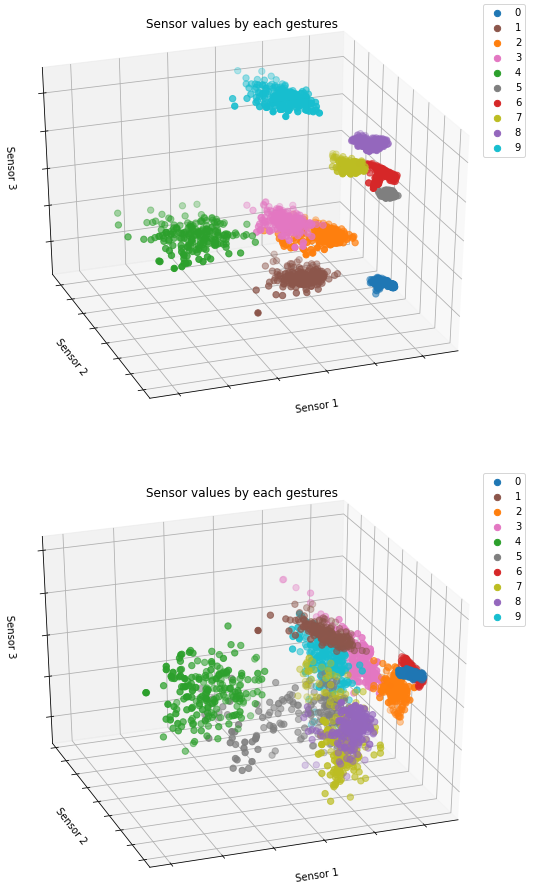
\includegraphics[width=6.8in]{Figures/pretty_f.png}
%   \caption{Collected 3-channel EMG sensor values for each different action}
%   \label{3dplot}
% \end{figure*}

\singlefigure[.9\textwidth]{3dplot}{pretty_f.png}{Collected 3-channel EMG sensor values for each different action}{Collected 3-channel EMG sensor values for each different action}

The evaluation results of the model are illustrated with a confusion
matrix as shown in Fig. \ref{cm}, which shows the accuracy per user
action label. Each column corresponds to the true label, which is the
user's intended hand gesture, and each row corresponds to the predicted
label, which is the gesture actuated by the prosthetic hand.

% \begin{figure}[h]
%   \centering
%   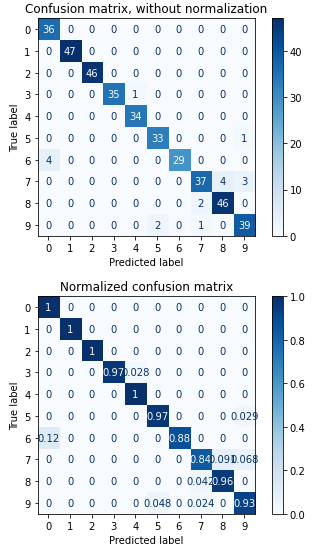
\includegraphics[width=3.1in]{Figures/confusionmatrix3.PNG}
%   \caption{Confusion matrix represents the accuracy per user action label}
%   \label{cm}
% \end{figure}

\singlefigure[.8\textwidth]{cm}{confusionmatrix3.PNG}{Confusion matrix represents the accuracy per user action label}{Confusion matrix represents the accuracy per user action label}

This equation \eqref{eq} is merely equivalent to the relationship of
predictions that the model classified precisely.

\begin{eqnarray}
  Accuracy & = & \frac{\textit{The number of correct predictions}}{\textit{Total number of predictions}} \\[1ex]
   & = & \frac{\textit{TP + TN}}{\textit{TP + TN + FP + FN}}
    \label{eq}
\end{eqnarray}


The average success rate for all subjects without noise was 94.96\% on
the training set and 91.58\% on the test-set. The best-case subject's
training set estimated accuracy was 95.69\% and the test set
estimated accuracy was 95.50\% as shown in Table 2. The impressive
point of this experiment was the unique gesture at the last part of
the experiment cycle.  As the last step of the experiment, users were
allowed to demonstrate any kind of creative unique gesture such as
crossed fingers, a V-for-victory sign, a finger gun, or the sign of
the horns.  The prosthetic hand successfully captured these gestures
with a high percentage (94\%).



\newcommand{\ra}[1]{\renewcommand{\arraystretch}{#1}}
% \begin{table}[h]
\tabcolsep=0.11cm
\begin{table*}
\footnotesize

\caption{Average recognition success rates of the trained RBF network, linear SVM network, and MLP network}
\centering
\ra{1.3}
\begin{tabular}{@{}rrrcrrcrr@{}}\toprule
\hline\hline %inserts double horizontal lines
& \multicolumn{2}{c}{$RBF$} & \phantom{abc}& \multicolumn{2}{c}{$Linear SVM$} &
\phantom{abc} & \multicolumn{2}{c}{$MLP$}\\
% \cmidrule{2-4} \cmidrule{6-8} \cmidrule{10-12}
$Subject$ & $Training$ $set$ & $Test$ $set$ && $Training$ $set$ & $Test$ $set$ && $Training$ $set$ & $Test$ $set$\\ \midrule
\hline
$without$ $noise$ $=$ $1$ & 95.69\% & 95.50\% && 88.25\% & 89.25\% && 90.50\% & 89.50\%\\
$2$ & 92.00\% & 90.00\% && 90.44\% & 89.50\% && 84.50\% & 84.50\%\\
$3$ & 97.19\% & 89.25\% && 89.19\% & 86.50\% && 87.44\% & 83.00\%\\
\hline
$with$ $noise$ $=$ $4$ & 92.06\% & 80.75\% && 79.25\% & 77.00\% && 68.38\% & 67.25\%\\
$5$ & 82.25\% & 80.50\% && 77.00\% & 73.50\% && 70.25\% & 68.50\%\\
$6$ & 88.44\% & 75.75\% && 68.94\% & 71.25\% && 65.06\% & 69.75\%\\
$7$ & 88.56\% & 83.25\% && 67.69\% & 67.50\% && 64.75\% & 62.25\%\\



\bottomrule
\hline
\end{tabular}

\end{table*}
% \end{table}

When measuring EMG sensors, sometimes sensor values bounce with
subjects' extreme actions.  This noise makes it difficult to obtain
sustainable high-quality electromyography signals for the long term
without tightening the sensor on the arm.  To record an undisturbed
sensor signal, a more elaborate connection apparatus is needed than
the prototype model possessed.  This would further improve the
system's accuracy.

As shown in Fig. \ref{chart3}, the average success rates with the
features extracted using the RBF kernel SVM classifier
\cite{ML1}\cite{ML2}, exhibit higher accuracy with reduced noise
levels.

% This results have much higher accuracy rather than 81.12\% obtained with Linear SVM classifier \cite{EEG}.

% \begin{figure}[h]
%   \centering
%   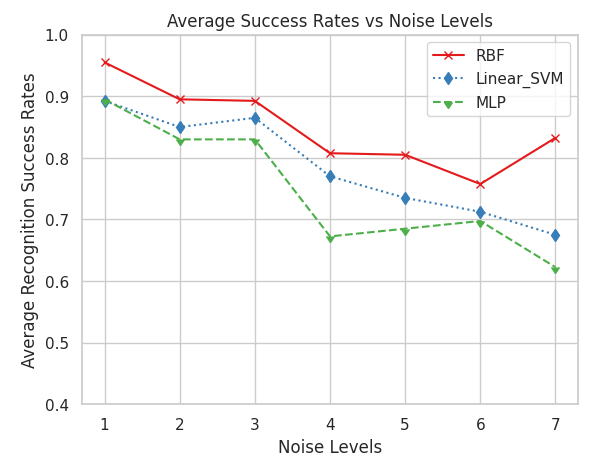
\includegraphics[width=3.3in]{Figures/chart_3.PNG}
%   \caption{Average recognition success rates of the trained RBF network, linear SVM network, and MLP network under different levels of noise inputs}
%   \label{chart3}
% \end{figure}

\singlefigure[.9\textwidth]{chart3}{chart_3.PNG}{Average recognition success rates of the trained RBF network, linear SVM network, and MLP network under different levels of noise inputs}{Average recognition success rates of the trained RBF network, linear SVM network, and MLP network under different levels of noise inputs}

This result demonstrates that applying user-customized training
software into the prosthetic hand can suffice for individual user
requirements with high performance.
